\chapter*{Introduction}
This master's thesis addresses the issue of mixing and its variations in the context of cooking as high-level tasks, taking into account contextual knowledge, in order to derive statements about which mixing movements a robotic agent should perform using a knowledge base.
Before we begin presenting the structure of the master's thesis, we would like to address five essential questions to provide readers with a better overview:
\begin{itemize}
    \item \textbf{What is the problem?} In the world of cooking and baking, various tasks need to be performed. While a human learns over their lifetime how to prepare recipes and intuitively execute the necessary actions, a robot must have these required actions readily available. A robot's tasks in the context of cooking can be diverse, such as cutting, pouring, or mixing. In this thesis, we focus on the task of mixing and examine the issue of different mixing actions and the context in which they are performed.    
    \item \textbf{Why is it important?} In the context of mixing, various movements need to be considered to achieve the desired results. It is not sufficient to consider a single movement as a general movement in the context of mixing, as different outcomes of a mixing action cannot be achieved otherwise. Therefore, different movements must be taken into account to achieve the desired results of a mixing action.
    \item \textbf{Why is it difficult?} At the current state of research, there is no systematic approach to determine which mixing movement should be performed under specific circumstances. Therefore, a systematic approach will be necessary, primarily utilizing video material. The challenge is to identify the relationships between the actions performed by humans, the ingredients used, and the associated movements. However, the biggest problem is deciding how to model this knowledge in a symbolic knowledge base so that the relevant knowledge is usable for the robot.
    \item \textbf{How is the problem solved?} Through the analysis of videos, we aim to determine how general principles can be inferred from individual cases, especially regarding human actions during the mixing of ingredients. We consider both the nature of the ingredients and the movements executed. The identified relationships will be modeled in a knowledge base, allowing a robotic agent to derive a possible movement with necessary parameters for execution. The knowledge base is symbolically modeled, enabling theoretical support for execution by many robotic agents.
    \item \textbf{How can this work contribute to research?} By implementing our knowledge base, it is possible for robotic agents to query the required knowledge for mixing actions. Our contribution is aimed at the development of robots capable of performing non-trivial tasks autonomously in household settings without having a predefined environment.
\end{itemize}


Our work is divided into multiple chapters that will cover every aspect of our research and practical work.
First, we intend to analyze existing research, particularly examining studies that delve into diverse mixing motions and exploring related systems that contain a queryable knowledge graph.
In the following section, we will introduce the reader with the frameworks employed to accomplish our objectives.	
Subsequently, we will present our approach to data acquisition and data representation.
In this chapter, we aim to explain the mixing tasks under consideration and articulate our methodology for representing this data to enable effective querying.
In the subsequent section, we will illustrate the implementation of our rules, with the ultimate aim of determining the appropriate motion to be employed.
To validate our concept, we have opted to simulate various scenarios and assess their outcomes, demonstrating the efficacy of our implemented system.
Before we will delve into the discussion of our results and draw conclusions to wrap up our work, we want to present a newly implemented web framework for graph visualization.

The following graphic is intended to provide an overview and will be referenced in each chapter to indicate which part of the work the chapter is addressing.
\begin{figure}[H]
    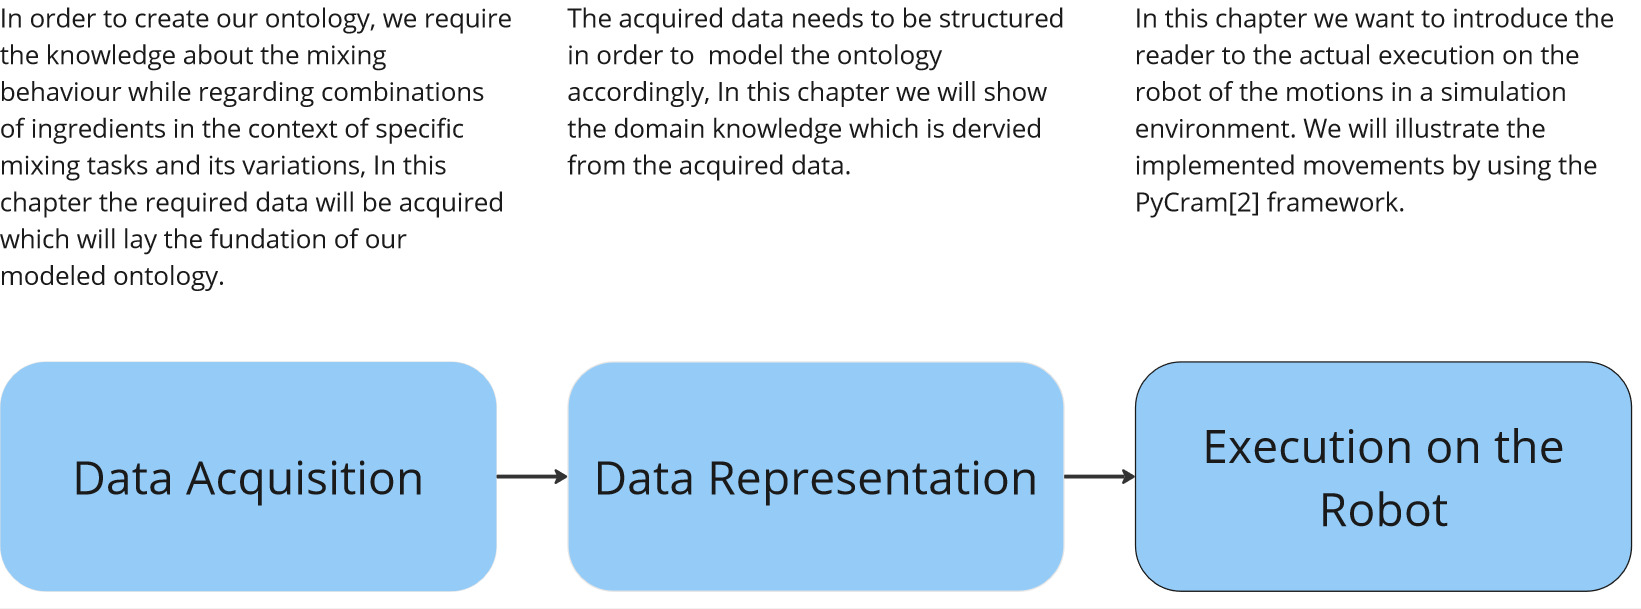
\includegraphics[scale=0.25]{Graphics/structure_overview.jpg}
\end{figure}